\section{重叠窗口拓扑扫描框架}\label{sec:method}

图~\ref{fig:flow}给出整体流程与统计冲突的来源：窗口是随机化单位，但重叠使原始观测被多个随机化单位共享。后续小节依次定义窗口构造、两种表示、最大扫描统计量与两种校准方法。

\begin{figure}[ht]
\centering
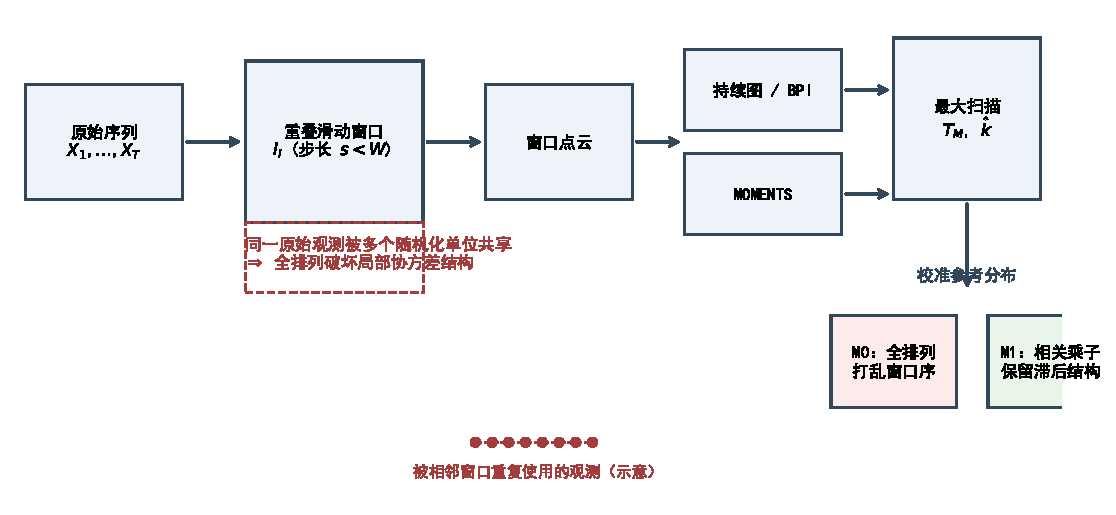
\includegraphics[width=0.95\textwidth]{../artifacts/figures/Figure1_method_schematic.pdf}
\caption{重叠窗口拓扑扫描与校准流程。原始序列经重叠窗口映射为窗口点云，再分别形成持续图/BPI 与矩表示 MOMENTS；最大扫描统计量给出检验统计量与位置估计；M0 对窗口顺序作全排列以构造参考分布，M1 使用相关乘子保留滞后依赖结构。虚线框标出被相邻窗口重复使用的原始观测：全排列重排窗口顺序时，原有的局部协方差结构被破坏，这是后文交换性失效机制的直观来源。}\label{fig:flow}
\end{figure}

\subsection{窗口构造与局部点云}\label{sec:windows}

给定观测序列 $X_1,\ldots,X_T$，取窗口宽度 $W$ 和步长 $s$，并令
\begin{equation}\label{eq:windows}
 a_i=(i-1)s+1,\qquad
 I_i=\{a_i,\ldots,a_i+W-1\},\qquad
 M=\left\lfloor\frac{T-W}{s}\right\rfloor+1.
\end{equation}
本文考虑 $1\le s\le W$，相邻窗口的名义重叠率为 $1-s/W$。对于二维观测，窗口点云直接定义为 $P_i=\{X_t:t\in I_i\}$。对于标量观测，在每个窗口内部构造三维时延点云
\begin{equation}\label{eq:delay-cloud}
 P_i=\bigl\{(X_t,X_{t+3},X_{t+6}):t=a_i,\ldots,a_i+W-7\bigr\},
\end{equation}
因而时延坐标不会跨越窗口边界。点云在计算持续同调前按固定规则进行精确去重；所有坐标尺度、网格、核宽和截断参数均预先设定，且不利用整条序列共同估计的自适应参数。该局部性条件将在第~\ref{sec:theory} 节用于界定窗口特征的依赖范围。

\subsection{固定网格持续强度表示}\label{sec:bpi}

对每个点云 $P_i$，在系数域 $\mathbb F_2$ 上计算 Vietoris--Rips 持续同调，并保留 0 维和 1 维同调通道中有限且寿命为正的 birth--death 对。相关计算框架和有限维表示可分别参见\cite{Bauer2021,Adams2017}。记第 $q\in\{0,1\}$ 个同调通道的持续图为
\[
 \mathcal D_i^{(q)}=\{(b_{ij}^{(q)},d_{ij}^{(q)})\}_j.
\]
给定场景固定的尺度上界 $c$，将每个有限持续图点转换为归一化 birth--lifetime 坐标
\begin{equation}\label{eq:bpi-normalization}
 u_{ij}^{(q)}=\min\left(\frac{b_{ij}^{(q)}}{c},1\right),\qquad
 v_{ij}^{(q)}=\min\left(\frac{d_{ij}^{(q)}-b_{ij}^{(q)}}{c},1\right).
\end{equation}
令 $\Delta=1/20$、$g_r=(r+1/2)\Delta$（$r=0,\ldots,19$）以及 $\sigma=0.05$。第 $q$ 个通道在网格中心 $(g_r,g_\ell)$ 上的持续强度坐标定义为
\begin{equation}\label{eq:bpi}
 Z_{i,r\ell}^{(q)}
 =\frac{\Delta}{2\pi\sigma^2}
 \sum_j v_{ij}^{(q)}
 \exp\left\{-\frac{(g_r-u_{ij}^{(q)})^2+(g_\ell-v_{ij}^{(q)})^2}{2\sigma^2}\right\}.
\end{equation}
每个同调通道产生 $20\times20=400$ 个坐标。按 0 维、1 维同调通道的顺序向量化并连接，再除以 $\sqrt 2$，得到 800 维特征
\begin{equation}\label{eq:bpi-vector}
 Y_i^{\mathrm{BPI}}
 =\frac{1}{\sqrt2}
 \begin{bmatrix}
   \operatorname{vec}(Z_i^{(0)})\\
   \operatorname{vec}(Z_i^{(1)})
 \end{bmatrix}.
\end{equation}
空通道记为 400 维零向量。N-AR 时延点云取 $c=6$，圆形模型及其备择取 $c=2.5$。为便于标识，本文将式\eqref{eq:bpi}--\eqref{eq:bpi-vector}所定义的固定网格持续强度向量记为 BPI。该算子在网格中心评价核强度，与对像素区域积分的某些 persistence-image 实现存在定义差异。

\subsection{矩表示}\label{sec:moments}

为构造低阶统计摘要作为对照，设窗口点云为 $P_i=\{x_{ij}\}_{j=1}^{n_i}\subset\mathbb R^d$，并定义
\begin{equation}\label{eq:moments}
 \bar x_i=\frac1{n_i}\sum_{j=1}^{n_i}x_{ij},\qquad
 S_i=\frac1{n_i}\sum_{j=1}^{n_i}(x_{ij}-\bar x_i)(x_{ij}-\bar x_i)^\top.
\end{equation}
MOMENTS 特征依次连接均值、协方差对角元以及按固定字典序排列的 $\sqrt2(S_i)_{ab}$（$a<b$）：
\begin{equation}\label{eq:moments-vector}
 Y_i^{\mathrm{MOM}}
 =\bigl(\bar x_i^\top,(S_i)_{11},\ldots,(S_i)_{dd},
 \{\sqrt2(S_i)_{ab}:a<b\}\bigr)^\top.
\end{equation}
其维数为 $d(d+3)/2$，故二维和三维点云分别得到 5 维和 9 维特征。$\sqrt2$ 权重保证任意两个窗口 $i,j$ 满足
\begin{equation}\label{eq:moments-frob}
 \|Y_i^{\mathrm{MOM}}-Y_j^{\mathrm{MOM}}\|_2^2
 =\|\bar x_i-\bar x_j\|_2^2+\|S_i-S_j\|_F^2.
\end{equation}
该表示主要概括一、二阶矩；有限窗口和序列依赖仍可能使其响应某些形状变化，因此本文不预设其对所有拓扑变化均不敏感。

\subsection{最大扫描统计量与位置估计}\label{sec:scan}

对任一窗口特征序列 $Y_1,\ldots,Y_M\in\mathbb R^p$，令
\begin{equation}\label{eq:bridge}
 U_M(k)=\frac1{\sqrt M}
 \left(\sum_{i=1}^kY_i-\frac{k}{M}\sum_{i=1}^M Y_i\right),
 \qquad t_k=\frac{k}{M},
\end{equation}
并定义标准化扫描曲线与最大统计量
\begin{equation}\label{eq:scan}
 Q_M(k)=\frac{\|U_M(k)\|_2^2}{t_k(1-t_k)},\qquad
 T_M=\max_{k\in\mathcal K_M}Q_M(k),
\end{equation}
其中
\[
 \mathcal K_M=\{\lceil0.15M\rceil,\ldots,M-\lceil0.15M\rceil\}.
\]
等价地，若 $\bar Y_{1:k}$ 和 $\bar Y_{k+1:M}$ 分别表示左右两段样本均值，则
\begin{equation}\label{eq:scan-equivalent}
 Q_M(k)=\frac{k(M-k)}{M}
 \|\bar Y_{1:k}-\bar Y_{k+1:M}\|_2^2.
\end{equation}

为使浮点并列情形具有确定性，令 $\epsilon_{64}=2^{-52}$，将满足
\[
 Q_M(k)\ge T_M-64\epsilon_{64}\max(1,|T_M|)
\]
的连续候选段定义为合格平台。位置估计选取最长平台；长度并列时取最左平台，再以该平台的下中位数作为 $\widehat k$。由于 $k$ 表示第 $k$ 与第 $k+1$ 个窗口之间的分割，映射到原始时间轴后的连续边界估计为
\begin{equation}\label{eq:location-map}
 \widehat\tau=\left(\widehat k-\frac12\right)s+\frac{W+1}{2}.
\end{equation}
若特征序列精确恒定，则规定 $T_M=0$。所有校准方法均使用相同的观测统计量、候选集合和位置规则。

\subsection{校准方法}\label{sec:calibration}

朴素置换方法记为 M0。条件于观测到的窗口特征，M0 对 $1,\ldots,M$ 作均匀随机排列，并在每个排列序列上重新计算式\eqref{eq:scan}。该方法保留经验边际分布，却不保留原始窗口顺序中的局部依赖。

依赖乘子自助法记为 M1。令 $\bar Y=M^{-1}\sum_{i=1}^M Y_i$、$Z_i=Y_i-\bar Y$，并取
\begin{equation}\label{eq:dmb-bandwidth}
 b=\max\left\{\left\lfloor\frac Ws\right\rfloor+1,
                 \left\lceil M^{1/3}\right\rceil\right\}.
\end{equation}
生成独立标准正态新息 $\varepsilon_1,\ldots,\varepsilon_{M+b-1}$，定义
\begin{equation}\label{eq:dmb-multiplier}
 \xi_i=b^{-1/2}\sum_{j=0}^{b-1}\varepsilon_{i+j},
 \qquad i=1,\ldots,M.
\end{equation}
由此
\begin{equation}\label{eq:dmb-cov}
 \operatorname{Cov}(\xi_i,\xi_{i+h})
 =\left(1-\frac{|h|}{b}\right)_+.
\end{equation}
M1 不作循环回绕，并对乘子加权序列 $\{\xi_iZ_i\}_{i=1}^M$ 应用与观测样本相同的桥接扫描。该构造属于依赖感知的参考近似；dependent wild bootstrap 和依赖乘子过程的一般理论可参见\cite{Shao2010,BucherKojadinovic2016}，其结论不直接构成本文完整 BPI 最大扫描的有限样本有效性定理。

两种方法均使用 $B=999$ 次重采样。若
\[
 K=\sum_{r=1}^{B}\mathbf 1\{T_{M,r}^*\ge T_M\},
\]
则 Monte Carlo $p$ 值定义为
\begin{equation}\label{eq:mc-pvalue}
 p=\frac{K+1}{B+1}=\frac{K+1}{1000}.
\end{equation}
本文以 $p\le0.05$ 拒绝零假设，等价于 $K\le49$。加一修正确保有限重采样下的 $p$ 值严格为正。
